\documentclass{article}
\usepackage{tikz-feynman}
\begin{document}
A manually placed Feynman diagram (no Lua needed):
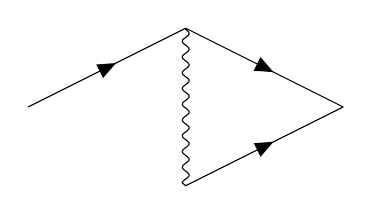
\begin{tikzpicture}
\begin{feynman}
\vertex (a) at (0, 0);
\vertex (b) at (2, 1);
\vertex (c) at (2, -1);
\vertex (d) at (4, 0);
\diagram*{(a) -- [fermion] (b) -- [fermion] (d),
  (b) -- [photon] (c),
  (c) -- [fermion] (d)};
\end{feynman}
\end{tikzpicture}
\end{document}
